% 第 7 章 游戏
\renewcommand{\codeInset}{63bp}
在第 6 章「增强 Qt 图形应用」中，我们用 Qt 图形库开发了一个模拟时钟、一个画图程序和一个编辑器。本章我们继续用 Qt 库开发奥赛罗棋（Othello，即黑白棋）和圈叉棋（Noughts and Crosses，即井字棋）这两个游戏。你可以在本篇引言之后找到对这两个游戏的介绍。本章我们从基本版本入手，由两名玩家互相对弈。在第 8 章「计算机对弈」中，我们将改进这两个游戏，让计算机与人类对弈。

本章将涵盖以下主题：

\begin{itemize}
\item 博弈论简介。我们开发一个游戏棋盘（game grid），玩家在其中轮流把自己的棋子加入棋盘。
\item 我们宣布获胜者。在奥赛罗棋中，每走一步之后，我们计算有多少对方的棋子可以被翻转。当棋盘的每个位置都被占据之后，我们宣布获胜者或平局。
\item 在圈叉棋中，我们统计一行中棋子的数量。如果一行中有五枚棋子，我们就宣布获胜者。
\item 我们继续使用类、字段和方法等 C++ 特性，也继续使用窗口和部件等 Qt 特性。
\end{itemize}

\section{奥赛罗棋}

在奥赛罗棋中，游戏开始时棋盘是空的。对局过程中，两名玩家轮流往棋盘上添加黑、白两色的棋子。每当一名玩家添加一枚棋子，我们就查看其他棋子，看看这枚新棋子是否把对方的某些棋子围住了。如果是，我们就把被围住的对方棋子换成己方的颜色。

例如，如果黑方玩家在一处位置添加一枚黑棋子，而该位置左边的三枚棋子是白色的、第四枚是黑色的，那么这三枚白色棋子就被这两枚黑色棋子围住了，它们会被换成黑色棋子。当棋盘上的每个位置都被黑色和白色棋子占满之后，我们统计棋子数量，拥有最多棋子的玩家获胜。如果黑色和白色棋子的数量相等，就是平局。

下面就是我们这个游戏应有的样子：

\begin{center}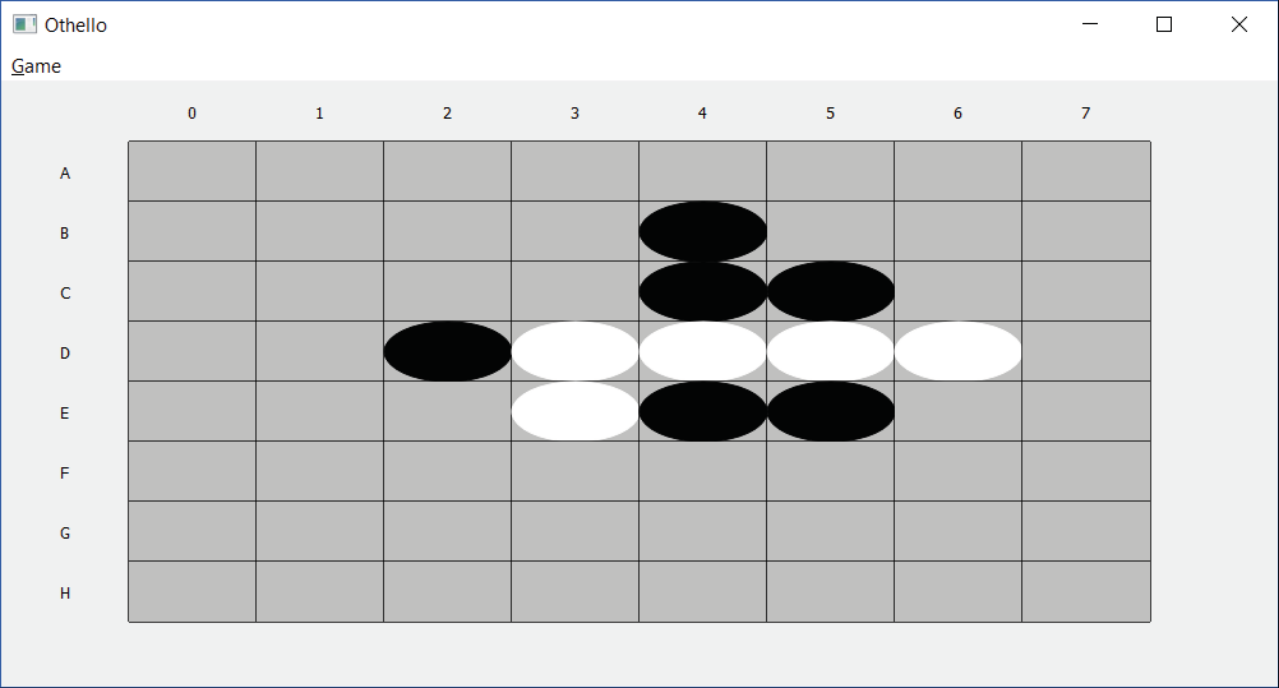
\includegraphics[width=0.9\textwidth]{images/p311_i04.png}\end{center}

\subsection{游戏部件}

首先，我们需要一个游戏棋盘。GameWidget 类是本章以及第 8 章「计算机对弈」中所有应用程序共有的。在第 5 章「Qt 图形应用」和第 6 章「增强 Qt 图形应用」中，我们开发的是 DocumentWidget 类，因为那时处理的是基于文档的应用程序。而在本章和第 8 章「计算机对弈」中，我们转而开发 GameWidget 类。

前两章的 DocumentWidget 类与本章及下一章的 GameWidget 类既有相似之处，也有不同之处。它们都是 Qt 类 QWidget 的子类，都打算嵌入到窗口中。不过，DocumentWidget 用来容纳文档，而 GameWidget 用来容纳游戏棋盘。它负责绘制棋盘，并捕获棋盘各个位置上的鼠标点击。GameWidget 是一个抽象类，让它的子类定义当用户点击鼠标时、或棋盘某个位置需要重绘时被调用的方法。

不过，我们复用前几章的 MainWindow 类来存放应用程序的主窗口及其菜单栏。

\medskip\noindent{\ttfamily\bfseries GameWidget.h}

\begin{codebox}
#ifndef GAMEWIDGET_H
#define GAMEWIDGET_H

#include <QPainter>
#include <QMouseEvent>
#include <QMessageBox>

#include "..\MainWindow\MainWindow.h"

class GameWidget : public QWidget {
  Q_OBJECT
\end{codebox}

构造函数初始化棋盘的行数和列数：

\begin{codebox}
  public:
    GameWidget(int rows, int columns, QWidget* parentWidget);
\end{codebox}

clearGrid 方法把棋盘中的每个位置都设为零，零被假定表示空位置。因此，每个继承 GameWidget 的类都应让零表示空位置：

\begin{codebox}
    void clearGrid();
\end{codebox}

当用户改变窗口大小时会调用 resizeEvent 方法。由于行数和列数是常数，每个位置的宽和高会按照窗口的新尺寸相应改变：

\begin{codebox}
    void resizeEvent(QResizeEvent *eventPtr);
\end{codebox}

当用户按下某个鼠标按钮时会调用 mousePressEvent，当窗口需要重绘时会调用 paintEvent，当用户点击窗口右上角的关闭框时会调用 closeEvent：

\begin{codebox}
    void mousePressEvent(QMouseEvent *eventPtr);
    void paintEvent(QPaintEvent *eventPtr);
    void closeEvent(QCloseEvent *eventPtr);
\end{codebox}

mouseMark 和 drawMark 方法是打算被子类重写的纯虚方法：当用户点击棋盘中的某个位置时会调用 mouseMark，当某个位置需要重绘时会调用 drawMark。它们是纯虚方法，GameWidget 因此是抽象的，这意味着 GameWidget 只能用作基类。GameWidget 的子类必须重写这些方法才能成为非抽象类：

\begin{codebox}
    virtual void mouseMark(int row, int column) = 0;
    virtual void drawMark(QPainter& painter,
                          const QRect& markRect, int mark) = 0;
\end{codebox}

isQuitOk 方法显示一个消息框，询问用户是否真的想退出对局：

\begin{codebox}
  private:
    bool isQuitOk();
\end{codebox}

在 Game 菜单变为可见之前会调用 isQuitEnabled 方法。当对局正在进行时，Quit 菜单项才被启用：

\begin{codebox}
  public slots:
    DEFINE_LISTENER(GameWidget, isQuitEnabled);
\end{codebox}

当用户选择 Quit 或 Exit 菜单项时会调用 onQuit 和 onExit 方法：

\begin{codebox}
    void onQuit();
    void onExit();
\end{codebox}

isGameInProgress 和 setGameInProgress 方法返回并设置 \texttt{m\_gameInProgress} 字段的值：

\begin{codebox}
  protected:
    bool isGameInProgress() const {return m_gameInProgress;}
    void setGameInProgress(bool active)
                          {m_gameInProgress = active;}
\end{codebox}

get 和 set 方法读取并设置棋盘中某个位置上的值。值是一个整数；记住，空位置被假定保存值零：

\begin{codebox}
  protected:
    int get(int row, int column) const;
    void set(int row, int column, int value);
\end{codebox}

只要对局正在进行，\texttt{m\_gameInProgress} 字段就为 true。\texttt{m\_rows} 和 \texttt{m\_columns} 字段保存棋盘的行数和列数；\texttt{m\_rowHeight} 和 \texttt{m\_columnWidth} 保存棋盘中每个位置以像素为单位的高度和宽度。最后，\texttt{m\_gameGrid} 是指向一个缓冲区的指针，缓冲区中保存着棋盘各个位置上的值：

\begin{codebox}
  private:
    bool m_gameInProgress = false;
    int m_rows, m_columns;
    int m_rowHeight, m_columnWidth;
    int* m_gameGrid;
};

#endif // GAMEWIDGET_H
\end{codebox}

GameWidget.cpp 文件存放 GameWidget 类各个方法的定义、鼠标事件方法、菜单方法，以及棋子的绘制和设置。

\medskip\noindent{\ttfamily\bfseries GameWidget.cpp}

\begin{codebox}
#include "GameWidget.h"
#include <QApplication>
#include <CAssert>
\end{codebox}

构造函数初始化棋盘的行数和列数，动态分配内存，并调用 clearGrid 来清空棋盘：

\begin{codebox}
GameWidget::GameWidget(int rows, int columns,
                       QWidget* parentWidget)
 :QWidget(parentWidget),
  m_rows(rows),
  m_columns(columns),
  m_gameGrid(new int[rows * columns]) {
  assert(rows > 0);
  assert(columns > 0);
  clearGrid();
}
\end{codebox}

get 方法返回行和列所指位置上的值，set 设置该值。保存值的缓冲区按行组织。也就是说，缓冲区的第一部分存放第一行，然后是第二行，依此类推：

\begin{codebox}
int GameWidget::get(int row, int column) const {
  return m_gameGrid[(row * m_columns) + column];
}

void GameWidget::set(int row, int column, int value) {
  m_gameGrid[(row * m_columns) + column] = value;
}
\end{codebox}

clearGrid 方法把每个位置都设为零，因为零被假定表示空位置：

\begin{codebox}
void GameWidget::clearGrid() {
  for (int row = 0; row < m_rows; ++row) {
    for (int column = 0; column < m_columns; ++column) {
      set(row, column, 0);
    }
  }
}
\end{codebox}

只要对局正在进行，Quit 菜单项就处于启用状态：

\begin{codebox}
bool GameWidget::isQuitEnabled() {
  return m_gameInProgress;
}
\end{codebox}

当用户选择退出对局时，如果对局正在进行，就会显示一个带有确认问题的消息框：

\begin{codebox}
bool GameWidget::isQuitOk() {
  if (m_gameInProgress) {
    QMessageBox messageBox(QMessageBox::Warning,
                           tr("Quit"), QString());
    messageBox.setText(tr("Quit the Game."));
    messageBox.setInformativeText
                  (tr("Do you really want to quit the game?"));
    messageBox.setStandardButtons(QMessageBox::Yes |
                                  QMessageBox::No);
    messageBox.setDefaultButton(QMessageBox::No);
\end{codebox}

如果用户按下 Yes 按钮，就返回 true：

\begin{codebox}
    return (messageBox.exec() == QMessageBox::Yes);
  }
\end{codebox}

如果没有对局正在进行，则不需要任何确认：

\begin{codebox}
  return true;
}
\end{codebox}

当用户选择 Quit 菜单项时会调用 onQuit 方法。如果对 isQuitOk 的调用返回 true，就把 \texttt{m\_gameInProgress} 设为 false，并调用 update，这最终会强制重绘窗口，从而清空棋盘。

\begin{codebox}
void GameWidget::onQuit() {
  if (isQuitOk()) {
    m_gameInProgress = false;
    update();
  }
}
\end{codebox}

当用户选择 Exit 菜单项时会调用 onExit 方法。如果对 isQuitOk 的调用返回 true，应用程序就退出。如下面的代码所示：

\begin{codebox}
void GameWidget::onExit() {
  if (isQuitOk()) {
    qApp->exit(0);
  }
}
\end{codebox}

当用户调整窗口大小时会调用 resizeEvent 方法。由于无论窗口大小如何，行数和列数都是常数，因此需要重新计算行高和列宽。我们把窗口的高度和宽度除以行数和列数加二，因为我们添加了额外的行和列作为边距。考虑下面的代码：

\begin{codebox}
void GameWidget::resizeEvent(QResizeEvent* eventPtr) {
  m_rowHeight = height() / (m_rows + 2);
  m_columnWidth = width() / (m_columns + 2);
  QWidget::resizeEvent(eventPtr);
  update();
}
\end{codebox}

当用户点击窗口时会调用 mousePressEvent 方法：

\begin{codebox}
void GameWidget::mousePressEvent(QMouseEvent* eventPtr) {
  if (m_gameInProgress &&
        (eventPtr->button() == Qt::LeftButton)) {
    QPoint mousePoint = eventPtr->pos();
\end{codebox}

由于棋盘被边距包围，需要从鼠标点中减去列宽和行高：

\begin{codebox}
    mousePoint.setX(mousePoint.x() - m_columnWidth);
    mousePoint.setY(mousePoint.y() - m_rowHeight);
\end{codebox}

如果鼠标点位于棋盘的某个位置之内，且该位置为空（零），就调用纯虚方法 mouseMark，由它负责鼠标点击的实际动作。在下一节中，会往棋盘添加黑色和白色棋子；在稍后的圈叉棋应用程序中，则会往棋盘添加圈和叉：

\begin{codebox}
    int row = mousePoint.y() / m_rowHeight,
       column = mousePoint.x() / m_columnWidth;
\end{codebox}

如果所点击的行和列位于棋盘之内（而不是棋盘外的边距中），且该位置为空（零），我们就以该行和列为参数调用纯虚方法 mouseMark：

\begin{codebox}
    if ((row < m_rows) && (column < m_columns) &&
        (get(row, column) == 0)) {
      mouseMark(row, column);
      update();
    }
  }
}
\end{codebox}

当窗口需要重绘时会调用 paintEvent 方法。如果对局正在进行（\texttt{m\_gameInProgress} 为 true），就写出各行和各列，然后对棋盘中的每个位置调用纯虚方法 drawMark，由它负责每个位置的实际绘制：

\begin{codebox}
void GameWidget::paintEvent(QPaintEvent* /*eventPtr*/) {
  if (m_gameInProgress) {
    QPainter painter(this);
    painter.setRenderHint(QPainter::Antialiasing);
    painter.setRenderHint(QPainter::TextAntialiasing);
\end{codebox}

首先，我们遍历各行，对每一行写出一个从 A 到 Z 的字母。字母表共有 26 个字母，我们假定行数不超过 26：

\begin{codebox}
    for (int row = 0; row < m_rows; ++row) {
      QString text;
      text.sprintf("%c", (char) (((int) 'A') + row));
      QRect charRect(0, (row + 1) * m_rowHeight,
                     m_columnWidth, m_rowHeight);
\end{codebox}

\begin{center}
\includegraphics[width=0.08\textwidth]{images/p318_i00.png}\end{center}

\begin{codebox}
      painter.drawText(charRect, Qt::AlignCenter |
                       Qt::AlignHCenter, text);
    }
\end{codebox}

然后我们遍历各列，对每一列写出它的编号：

\begin{codebox}
    for (int column = 0; column < m_columns; ++column) {
      QString text;
      text.sprintf("%i", column);
      QRect charRect((column + 1) * m_columnWidth, 0,
                     m_columnWidth, m_rowHeight);
      painter.drawText(charRect, Qt::AlignCenter |
                       Qt::AlignHCenter, text);
    }

    painter.save();
    painter.translate(m_columnWidth, m_rowHeight);
\end{codebox}

\begin{myNotic}{p028_i00}{纯虚方法是不打算在类本身中定义、而只打算在其子类中定义的方法。持有至少一个纯虚方法的类将成为抽象类，这意味着无法创建该类的对象。这样的类只能用作类层次结构中的基类。继承抽象类的类必须定义基类的每一个纯虚方法，否则它自己也会成为抽象类。}
\end{myNotic}

最后，我们遍历棋盘，对每个位置，以该位置的矩形和它当前的棋子为参数调用纯虚方法 drawMark：

\begin{codebox}
    for (int row = 0; row < m_rows; ++row) {
      for (int column = 0; column < m_columns; ++column) {
        QRect markRect(column * m_columnWidth, row * m_rowHeight,
                       m_columnWidth, m_rowHeight);
        painter.setPen(Qt::black);
        painter.drawRect(markRect);
        painter.fillRect(markRect, Qt::lightGray);
        drawMark(painter, markRect, get(row, column));
      }
    }

    painter.restore();
  }
}
\end{codebox}

当用户点击窗口右上角的关闭框时会调用 closeEvent 方法。如果对 isQuitOk 的调用返回 true，窗口就关闭，应用程序退出：

\begin{codebox}
void GameWidget::closeEvent(QCloseEvent* eventPtr) {
  if (isQuitOk()) {
    eventPtr->accept();
    qApp->exit(0);
  }
  else {
    eventPtr->ignore();
  }
}
\end{codebox}

\subsubsection{OthelloWindow 类}

OthelloWindow 类继承自第 6 章「增强 Qt 图形应用」的 MainWindow。它向窗口添加菜单，并把 OthelloWidget 类——GameWidget 的一个子类——设为窗口的中心部件。

\medskip\noindent{\ttfamily\bfseries OthelloWindow.h}

\begin{codebox}
#ifndef OTHELLOWINDOW_H
#define OTHELLOWINDOW_H

#include "..\MainWindow\MainWindow.h"
#include "OthelloWidget.h"

class OthelloWindow : public MainWindow {
  Q_OBJECT

  public:
    OthelloWindow(QWidget *parentWidget = nullptr);
    ~OthelloWindow();

    void closeEvent(QCloseEvent *eventPtr)
      {m_othelloWidgetPtr->closeEvent(eventPtr);}
\end{codebox}

\texttt{m\_othelloWidgetPtr} 字段保存指向窗口中心部件的指针。它指向一个 OthelloWidget 类的对象：

\begin{codebox}
  private:
    OthelloWidget* m_othelloWidgetPtr;
};

#endif // OTHELLOWINDOW_H
\end{codebox}

OthelloWindow.cpp 文件存放 OthelloWindow 类各个方法的定义。

\medskip\noindent{\ttfamily\bfseries OthelloWindow.cpp}

\begin{codebox}
#include "OthelloWidget.h"
#include "OthelloWindow.h"
#include <QtWidgets>
\end{codebox}

构造函数把窗口的标题设为 Othello，并把大小设为 1000 $\times$ 500 像素：

\begin{codebox}
OthelloWindow::OthelloWindow(QWidget *parentWidget /*= nullptr*/)
 :MainWindow(parentWidget) {
  setWindowTitle(tr("Othello"));
  resize(1000, 500);
\end{codebox}

一个 OthelloWidget 对象被动态创建，并放在窗口的中心：

\begin{codebox}
  m_othelloWidgetPtr = new OthelloWidget(this);
  setCentralWidget(m_othelloWidgetPtr);
\end{codebox}

我们向菜单栏添加 Game 菜单，并把 onMenuShow 方法连接到该菜单，使得它在菜单变为可见之前被调用：

\begin{codebox}
  { QMenu* gameMenuPtr = menuBar()->addMenu(tr("&Game"));
    connect(gameMenuPtr, SIGNAL(aboutToShow()),
            this, SLOT(onMenuShow()));
\end{codebox}

用户可以选择黑色或白色来先走。在菜单项变为可见之前会调用 isBlackStartsEnabled 和 isWhiteStartsEnabled 方法。当对局正在进行时，菜单项被禁用：

\begin{codebox}
    addAction(gameMenuPtr, tr("&Black Starts"),
              SLOT(onBlackStarts()), 0,
              tr("Black Starts"), nullptr,tr("Black Starts"),
              LISTENER(isBlackStartsEnabled));

    addAction(gameMenuPtr, tr("&White Starts"),
              SLOT(onWhiteStarts()), 0,
              tr("White Starts"), nullptr, tr("White Starts"),
              LISTENER(isWhiteStartsEnabled));

    gameMenuPtr->addSeparator();
\end{codebox}

当对局正在进行时，用户可以退出对局。当没有对局正在进行时，该菜单项被禁用：

\begin{codebox}
    addAction(gameMenuPtr, tr("&Quit the Game"),
              SLOT(onQuit()),
              QKeySequence(Qt::CTRL + Qt::Key_Q),
              tr("Quit Game"), nullptr, tr("Quit the Game"),
              LISTENER(isQuitEnabled));
\end{codebox}

用户可以随时退出应用程序：

\begin{codebox}
    addAction(gameMenuPtr, tr("E&xit"),
              SLOT(onExit()), QKeySequence::Quit);
  }
}
\end{codebox}

析构函数释放窗口中心的奥赛罗部件：

\begin{codebox}
OthelloWindow::~OthelloWindow() {
  delete m_othelloWidgetPtr;
}
\end{codebox}

\subsubsection{OthelloWidget 类}

OthelloWidget 是本章开头定义的 GameWidget 类的子类。它通过重写 mouseMark 和 drawMark 成为非抽象类：当用户点击棋盘中的某个位置时会调用 mouseMark，当某个位置需要重绘时会调用 drawMark。

\medskip\noindent{\ttfamily\bfseries OthelloWidget.h}

\begin{codebox}
#ifndef OTHELLOWIDGET_H
#define OTHELLOWIDGET_H

#include "..\MainWindow\GameWidget.h"

#define ROWS    8
#define COLUMNS 8
\end{codebox}

奥赛罗棋中的棋子可以是黑色或白色。我们使用 Mark 枚举来保存棋盘上的值。Empty 项的值为零，而 GameWidget 假定零表示空位置：

\begin{codebox}
enum Mark {Empty = 0, Black, White};

class OthelloWidget : public GameWidget {
\end{codebox}

\begin{codebox}
  Q_OBJECT

  public:
    OthelloWidget(QWidget* parentWidget);

    void mouseMark(int row, int column);
    void drawMark(QPainter& painter,
                  const QRect& markRect, int mark);
\end{codebox}

在 BlackStarts 和 WhiteStarts 菜单项变为可见之前会调用 isBlackStartsEnabled 和 isWhiteStartsEnabled 监听器，以决定是否启用它们。注意，监听器和方法必须标记为 public slots，菜单框架才会把它们当作监听器：

\begin{codebox}
  public slots:
    DEFINE_LISTENER(OthelloWidget, isBlackStartsEnabled);
    DEFINE_LISTENER(OthelloWidget, isWhiteStartsEnabled);
\end{codebox}

当用户选择 BlackStarts 和 WhiteStarts 菜单项时会调用 onBlackStarts 和 onWhiteStarts 方法：

\begin{codebox}
    void onBlackStarts();
    void onWhiteStarts();
\end{codebox}

checkWinner 方法检查棋盘上的每个位置是否都已被黑色或白色棋子占据。如果是，就统计棋子，并宣布获胜者，除非是平局：

\begin{codebox}
  private:
    void checkWinner();
\end{codebox}

turn 方法在其中一名玩家走了一步之后被调用。它计算这次走法将要翻转的位置：

\begin{codebox}
    void turn(int row, int column, Mark mark);
\end{codebox}

calculateMark 方法计算如果玩家把棋子放在行和列所指定的位置，需要翻转的棋子集合：

\begin{codebox}
    void calculateMark(int row, int column, Mark mark,
                       QSet<QPair<int,int>>& resultSet);
\end{codebox}

\texttt{m\_nextMark} 字段交替取前述 Mark 枚举中的 Black 和 White 值，取决于接下来要由哪位玩家走棋。它由 onBlackStarts 或 onWhiteStarts 初始化，如前面的代码所示：

\begin{codebox}
  Mark m_nextMark;
};

#endif // OTHELLOWIDGET_H
\end{codebox}

OthelloWidget 类持有对局的功能。它允许玩家往棋盘添加黑色和白色棋子、翻转棋子，并宣布获胜者。

\medskip\noindent{\ttfamily\bfseries OthelloWidget.cpp}

\begin{codebox}
#include "OthelloWidget.h"
#include "OthelloWindow.h"

#include <QTime>
#include <CTime>
#include <CAssert>
using namespace std;

OthelloWidget::OthelloWidget(QWidget* parentWidget)
 :GameWidget(ROWS, COLUMNS, parentWidget) {
  // Empty.
}
\end{codebox}

当对局尚未开始时，BlackStarts 和 WhiteStarts 菜单项处于启用状态：

\begin{codebox}
bool OthelloWidget::isBlackStartsEnabled() {
  return !isGameInProgress();
}

bool OthelloWidget::isWhiteStartsEnabled() {
  return !isGameInProgress();
}
\end{codebox}

onBlackStarts 和 onWhiteStarts 方法开始一局新对局，设置先走的那枚棋子（黑色或白色），清空棋盘，并更新窗口以绘制一个空的棋盘：

\begin{codebox}
void OthelloWidget::onBlackStarts() {
  setGameInProgress(true);
  m_nextMark = Black;
  update();
}

void OthelloWidget::onWhiteStarts() {
  setGameInProgress(true);
  m_nextMark = White;
  update();
}
\end{codebox}

当玩家点击棋盘中的一个空位置时会调用 mouseMark 方法。我们用下一枚棋子设置该位置，翻转受这次走法影响的每一枚棋子，并更新窗口以反映变化：

\begin{codebox}
void OthelloWidget::mouseMark(int row, int column) {
  set(row, column, m_nextMark);
  turn(row, column, m_nextMark);
  update();
\end{codebox}

我们检查这次走法是否使棋盘填满，并切换下一枚棋子：

\begin{codebox}
  checkWinner();
  m_nextMark = (m_nextMark == Black) ? White : Black;
}
\end{codebox}

当棋盘中的某个位置需要重绘时会调用 drawMark 方法。如果该位置不为空，我们就绘制一个带黑色边框的黑色或白色椭圆。如果位置为空，我们什么也不做。注意，框架会在调用重绘之前清空窗口：

\begin{codebox}
void OthelloWidget::drawMark(QPainter& painter,
     const QRect& markRect, int mark) {
  painter.setPen(Qt::black);
  painter.drawRect(markRect);
  painter.fillRect(markRect, Qt::lightGray);

  switch (mark) {
    case Black:
      painter.setPen(Qt::black);
      painter.setBrush(Qt::black);
      painter.drawEllipse(markRect);
      break;

    case White:
      painter.setPen(Qt::white);
      painter.setBrush(Qt::white);
      painter.drawEllipse(markRect);
      break;

    case Empty:
      break;
  }
}
\end{codebox}

checkWinner 方法统计被黑色和白色棋子占据的位置数量以及空位置的数量：

\begin{codebox}
void OthelloWidget::checkWinner() {
  int blacks = 0, whites = 0, empties = 0;

  for (int row = 0; row < ROWS; ++row) {
    for (int column = 0; column < COLUMNS; ++column) {
      switch (get(row, column)) {
        case Black:
          ++blacks;
          break;

        case White:
          ++whites;
          break;

        case Empty:
          ++empties;
          break;
      }
    }
  }
\end{codebox}

如果没有空位置剩下，对局就结束了，我们宣布获胜者，除非是平局。获胜者是拥有最多己方颜色棋子的玩家：

\begin{codebox}
  if (empties == 0) {
    QMessageBox messageBox(QMessageBox::Information,
        tr("Victory"), QString());
    QString text;

    if (blacks == whites) {
      text.sprintf("A Draw.");
    }
    else if (blacks > whites) {
      text.sprintf("The Winner: Black");
    }
    else {
      text.sprintf("The Winner: White");
    }

    messageBox.setText(text);
    messageBox.setStandardButtons(QMessageBox::Ok);
    messageBox.exec();
    setGameInProgress(false);

    clearGrid();
    update();
  }
}
\end{codebox}

turn 方法调用 calculateMark 来获得需要翻转棋子的位置集合。然后，集合中的每个位置都被设为相应的棋子。

在这个应用程序中，turn 是唯一调用 calculateMark 的方法。然而，在第 8 章「计算机对弈」中，calculateMark 还会被调用来计算计算机玩家的走法。因此，turn 和 calculateMark 的功能被分成了两个方法：

\begin{codebox}
void OthelloWidget::turn(int row, int column, Mark mark) {
  QSet<QPair<int,int>> totalSet;
  calculateMark(row, column, mark, totalSet);

  for (QPair<int,int> pair : totalSet) {
    int row = pair.first, column = pair.second;
    set(row, column, mark);
  }
}
\end{codebox}

calculateMark 方法统计棋盘中每个位置在所有八个方向上将翻转的棋子数量：

\begin{codebox}
void OthelloWidget::calculateMark(int row, int column,
    Mark playerMark, QSet<QPair<int,int>>& totalSet){
\end{codebox}

\texttt{directionArray} 中的每个整数对都按照罗盘方位对应一个方向：

\begin{codebox}
  QPair<int,int> directionArray[] =
    {QPair<int,int>(-1, 0),   // 北
     QPair<int,int>(-1, 1),   // 东北
     QPair<int,int>(0, 1),    // 东
     QPair<int,int>(1, 1),    // 东南
     QPair<int,int>(1, 0),    // 南
     QPair<int,int>(1, -1),   // 西南
     QPair<int,int>(0, -1),   // 西
     QPair<int,int>(-1, -1)}; // 西北
\end{codebox}

数组的大小可以用数组的总大小（以字节为单位）除以第一个值的大小来确定：

\begin{codebox}
  int arraySize =
    (sizeof directionArray) / (sizeof directionArray[0]);
\end{codebox}

我们遍历各个方向；对每个方向，只要找到的是对方的棋子，就沿该方向继续移动：

\begin{codebox}
  for (int index = 0; index < arraySize; ++index) {
    QPair<int,int> pair = directionArray[index];
\end{codebox}

在沿该方向迭代的过程中，row 和 column 字段保存当前的行和列：

\begin{codebox}
    int rowStep = pair.first, columnStep = pair.second,
        currRow = row, currColumn = column;
\end{codebox}

我们把迭代过程中找到的棋子收集在 \texttt{directionSet} 中：

\begin{codebox}
    QSet<QPair<int,int>> directionSet;

    while (true) {
      currRow += rowStep;
      currColumn += columnStep;
\end{codebox}

如果我们到达棋盘的某条边界，或者找到空位置，就中断迭代：

\begin{codebox}
      if ((currRow < 0) || (currRow == ROWS) ||
          (currColumn < 0) || (currColumn == COLUMNS) ||
          (get(currRow, currColumn) == Empty)) {
        break;
      }
\end{codebox}

如果我们找到玩家的棋子，就把方向集合并入总集合，并中断迭代：

\begin{codebox}
      else if (get(currRow, currColumn) == playerMark) {
        totalSet += directionSet;
        break;
      }
\end{codebox}

如果我们既没有找到玩家的棋子，也没有找到空位置，那么找到的就是对方的棋子，我们就把它的位置加入方向集合：

\begin{codebox}
      else {
        directionSet.insert(QPair<int,int>(row, column));
      }
    }
  }
}
\end{codebox}

\subsubsection{main 函数}

\texttt{main} 函数的工作方式与前面的 Qt 应用程序相同。它创建一个应用程序，显示奥赛罗棋窗口，并执行应用程序。执行一直持续到 exit 方法被调用——当用户关闭窗口或选择 Exit 菜单项时就会调用它。

\medskip\noindent{\ttfamily\bfseries Main.cpp}

\begin{codebox}
#include "OthelloWidget.h"
#include "OthelloWindow.h"
#include <QApplication>

int main(int argc, char *argv[]) {
  QApplication application(argc, argv);
  OthelloWindow othelloWindow;
  othelloWindow.show();
  return application.exec();
}
\end{codebox}

\section{圈叉棋}

圈叉棋应用程序搭建一个游戏棋盘，并允许两名玩家互相对弈。在圈叉棋中，两名玩家轮流往棋盘上添加圈和叉。最先成功把五枚棋子排成一行者获胜。棋子可以水平、垂直或沿对角线放置。当每名玩家试图把自己的五枚棋子排成一行时，也必须设法阻止对方排出五子。

在第 8 章「计算机对弈」中，计算机将与人类对弈。

\subsection{NaCWindow 类}

我们复用游戏部件一节中的 GameWidget。NaCWindow 类与 OthelloWindow 类相似。它向窗口的菜单栏添加 Nought Starts 和 Cross Starts 菜单项。

\medskip\noindent{\ttfamily\bfseries NaCWindow.h}

\begin{codebox}
#ifndef NACWINDOW_H
#define NACWINDOW_H

#include "..\MainWindow\MainWindow.h"
#include "NaCWidget.h"

class NaCWindow : public MainWindow {
  Q_OBJECT

  public:
    NaCWindow(QWidget *parentWidget = nullptr);
    ~NaCWindow();

  public:
    void closeEvent(QCloseEvent *eventPtr) override
                   {m_nacWidgetPtr->closeEvent(eventPtr);}

  private:
    NaCWidget* m_nacWidgetPtr;
};

#endif // NACWINDOW_H
\end{codebox}

NaCWindow.cpp 文件存放 NaCWindow 类各个方法的定义。

\medskip\noindent{\ttfamily\bfseries NaCWindow.cpp}

\begin{codebox}
#include "NaCWindow.h"
#include <QtWidgets>

NaCWindow::NaCWindow(QWidget *parentWidget /*= nullptr*/)
 :MainWindow(parentWidget) {
  setWindowTitle(tr("Noughts and Crosses"));
  resize(1000, 500);

  m_nacWidgetPtr = new NaCWidget(this);
  setCentralWidget(m_nacWidgetPtr);

  { QMenu* gameMenuPtr = menuBar()->addMenu(tr("&Game"));
\end{codebox}

\begin{codebox}
    connect(gameMenuPtr, SIGNAL(aboutToShow()),
            this, SLOT(onMenuShow()));

    addAction(gameMenuPtr, tr("&Nought Starts"),
              SLOT(onNoughtStarts()), 0,
              tr("Nought Starts"), nullptr, tr("Nought Starts"),
              LISTENER(isNoughtStartsEnabled));

    addAction(gameMenuPtr, tr("&Cross Starts"),
              SLOT(onCrossStarts()), 0,
              tr("Cross Starts"), nullptr, tr("Cross Starts"),
              LISTENER(isCrossStartsEnabled));

    gameMenuPtr->addSeparator();

    addAction(gameMenuPtr, tr("&Quit the Game"),
              SLOT(onQuit()),
              QKeySequence(Qt::CTRL + Qt::Key_Q), tr("Quit Game"),
              nullptr, tr("Quit the Game"),
              LISTENER(isQuitEnabled));

    addAction(gameMenuPtr, tr("E&xit"),
              SLOT(onExit()), QKeySequence::Quit);
  }
}

NaCWindow::~NaCWindow() {
  delete m_nacWidgetPtr;
}
\end{codebox}

\subsubsection{NaCWidget 类}

NaCWidget 类处理圈叉棋的功能。它允许两名玩家互相对弈。在第 8 章「计算机对弈」中，我们将编写一个计算机与人类对弈的游戏。

\medskip\noindent{\ttfamily\bfseries NaCWidget.h}

\begin{codebox}
#ifndef NACWIDGET_H
#define NACWIDGET_H

#include "..\MainWindow\GameWidget.h"

#define ROWS    26
#define COLUMNS 26
\end{codebox}

与奥赛罗棋应用程序类似，棋盘中的一个位置可以保存三个值之一：

\begin{itemize}
\item Empty（即零）；
\item Nought（圈）；
\item Cross（叉）。
\end{itemize}

Mark 枚举对应 Empty、Nought 和 Cross 这三个值：

\begin{codebox}
enum Mark {Empty = 0, Nought, Cross};

class NaCWidget : public GameWidget {
  Q_OBJECT

  public:
    NaCWidget(QWidget* parentWidget);

    void mouseMark(int row, int column);
    void drawMark(QPainter& painter,
                  const QRect& markRect, int mark);

  public slots:
    DEFINE_LISTENER(NaCWidget, isNoughtStartsEnabled);
    void onNoughtStarts();

    DEFINE_LISTENER(NaCWidget, isCrossStartsEnabled);
    void onCrossStarts();

  private:
    void checkWinner(int row, int column, Mark mark);
    int countMarks(int row, int column, int rowStep,
                   int columnStep, Mark mark);

    Mark m_nextMark;
};

#endif // NACWIDGET_H
\end{codebox}

NaCWidget.cpp 文件存放 NaCWidget 类各个方法的定义。

\medskip\noindent{\ttfamily\bfseries NaCWidget.cpp}

\begin{codebox}
#include "NaCWidget.h"
#include <CTime>

NaCWidget::NaCWidget(QWidget* parentWidget)
 :GameWidget(ROWS, COLUMNS, parentWidget) {
  // Empty.
}
\end{codebox}

在 Game 菜单变为可见之前会调用 isNoughtStartsEnabled 和 isCrossStartsEnabled 方法。当没有对局正在进行时，Nought Starts 和 Cross Starts 菜单项处于启用状态：

\begin{codebox}
bool NaCWidget::isCrossStartsEnabled() {
  return !isGameInProgress();
}

bool NaCWidget::isNoughtStartsEnabled() {
  return !isGameInProgress();
}
\end{codebox}

当用户选择 Nought Starts 和 Cross Starts 菜单项时会调用 onNoughtStarts 和 onCrossStarts 方法。它们把对局设为进行中，设置用来先走的那枚棋子（\texttt{m\_nextMark}），并通过调用 update 强制重绘棋盘：

\begin{codebox}
void NaCWidget::onNoughtStarts() {
  setGameInProgress(true);
  m_nextMark = Nought;
  update();
}

void NaCWidget::onCrossStarts() {
  setGameInProgress(true);
  m_nextMark = Cross;
  update();
}
\end{codebox}

当玩家点击棋盘中的某个位置时会调用 mouseMark 方法。我们在该位置设置下一枚棋子，检查是否有玩家赢得了对局，交换下一手棋，并通过调用 update 重绘窗口：

\begin{codebox}
void NaCWidget::mouseMark(int row, int column) {
  set(row, column, m_nextMark);
  checkWinner(row, column, m_nextMark);
  m_nextMark = (m_nextMark == Nought) ? Cross : Nought;
  update();
}
\end{codebox}

当棋盘中的某个位置需要重绘时会调用 drawMark 方法：

\begin{codebox}
void NaCWidget::drawMark(QPainter& painter,
    const QRect& markRect, int mark) {
\end{codebox}

我们把画笔颜色设为黑色；如果是圈，就画一个椭圆，如下所示：

\begin{codebox}
  painter.setPen(Qt::black);
  switch (mark) {
    case Nought:
      painter.drawEllipse(markRect);
      break;
\end{codebox}

如果是叉，我们就画两条直线，分别连接左上角和右下角、右上角和左下角：

\begin{codebox}
    case Cross:
      painter.drawLine(markRect.topLeft(),
                       markRect.bottomRight());
      painter.drawLine(markRect.topRight(),
                       markRect.bottomLeft());
      break;
\end{codebox}

如果是空位置，我们什么也不做。记住，框架会在重绘之前清空窗口：

\begin{codebox}
    case Empty:
      break;
  }
}
\end{codebox}

当一名玩家走了一步之后，我们检查这次走法是否导致了胜利。我们在四个方向上调用 countMarks 来做 checkWinner，看看这次走法是否造成了五枚棋子连成一行：

\begin{codebox}
void NaCWidget::checkWinner(int row, int column, Mark mark) {
\end{codebox}

南北方向的代码是：

\begin{codebox}
  if ((countMarks(row, column, -1, 0, mark) >= 5) ||
\end{codebox}

东西方向的代码是：

\begin{codebox}
      (countMarks(row, column, 0, -1, mark) >= 5) ||
\end{codebox}

西北—东南方向的代码是：

\begin{codebox}
      (countMarks(row, column, -1, 1, mark) >= 5) ||
\end{codebox}

东南—西北方向的代码是：

\begin{codebox}
      (countMarks(row, column, 1, 1, mark) >= 5)) {
\end{codebox}

如果这次走法造成了五子连珠，我们就显示一个带有获胜者（圈或叉）的消息框。在圈叉棋中不会有平局：

\begin{codebox}
    QMessageBox messageBox(QMessageBox::Information,
                           tr("Victory"), QString());
    QString text;
    text.sprintf("The Winner: %s.",
                 (mark == Nought) ? "Nought" : "Cross");

    messageBox.setText(text);
    messageBox.setStandardButtons(QMessageBox::Ok);
    messageBox.exec();
    setGameInProgress(false);
\end{codebox}

棋盘被清空，从而准备好下一局对局：

\begin{codebox}
    clearGrid();
    update();
  }
}
\end{codebox}

countMarks 方法统计一行中棋子的数量。我们在两个方向上都调用 countMarks。例如，如果 \texttt{rowStep} 和 \texttt{columnStep} 都是负一，我们就在每次迭代中把当前行和当前列都减一。这意味着第一次迭代时我们在东北方向上调用 countMarks。第二次迭代时，我们在相反的方向上调用 countMarks，也就是西南方向：

\begin{codebox}
int NaCWidget::countMarks(int row, int column, int rowStep,
                          int columnStep, Mark mark) {
  int countMarks = 0;
\end{codebox}

我们会一直计数，直到遇到棋盘的某条边界，或者找到一枚不是我们正在计数的棋子——也就是说，是对方的棋子或一枚空棋子：

\begin{codebox}
  { int currentRow = row, currentColumn = column;
    while ((currentRow >= 0) && (currentRow < ROWS) &&
           (currentColumn >= 0) && (currentColumn < COLUMNS) &&
           (get(currentRow, currentColumn) == mark)) {
      ++countMarks;
      currentRow += rowStep;
      currentColumn += columnStep;
    }
  }
\end{codebox}

在第二次迭代中，我们不是加上行和列的步长，而是减去它们。这样，我们就在相反的方向上调用 countMarks。我们还通过加上步长来初始化当前的行和列，这样就不会把中间那枚棋子计数两次：

\begin{codebox}
  { int currentRow = row + rowStep,
        currentColumn = column + columnStep;
    while ((currentRow >= 0) && (currentRow < ROWS) &&
         (currentColumn >= 0) && (currentColumn < COLUMNS) &&
         (get(currentRow, currentColumn) == mark)) {
      ++countMarks;
      currentRow -= rowStep;
      currentColumn -= columnStep;
    }
  }

  return countMarks;
}
\end{codebox}

\subsubsection{main 函数}

\texttt{main} 函数创建应用程序，显示窗口，并执行应用程序，直到用户关闭窗口或选择 Exit 菜单项。

\medskip\noindent{\ttfamily\bfseries Main.cpp}

\begin{codebox}
#include "NaCWidget.h"
#include "NaCWindow.h"
#include <QApplication>

int main(int argc, char *argv[]) {
  QApplication application(argc, argv);
  NaCWindow mainWindow;
  mainWindow.show();
  return application.exec();
}
\end{codebox}

运行前面的代码后，输出如下所示：

\begin{center}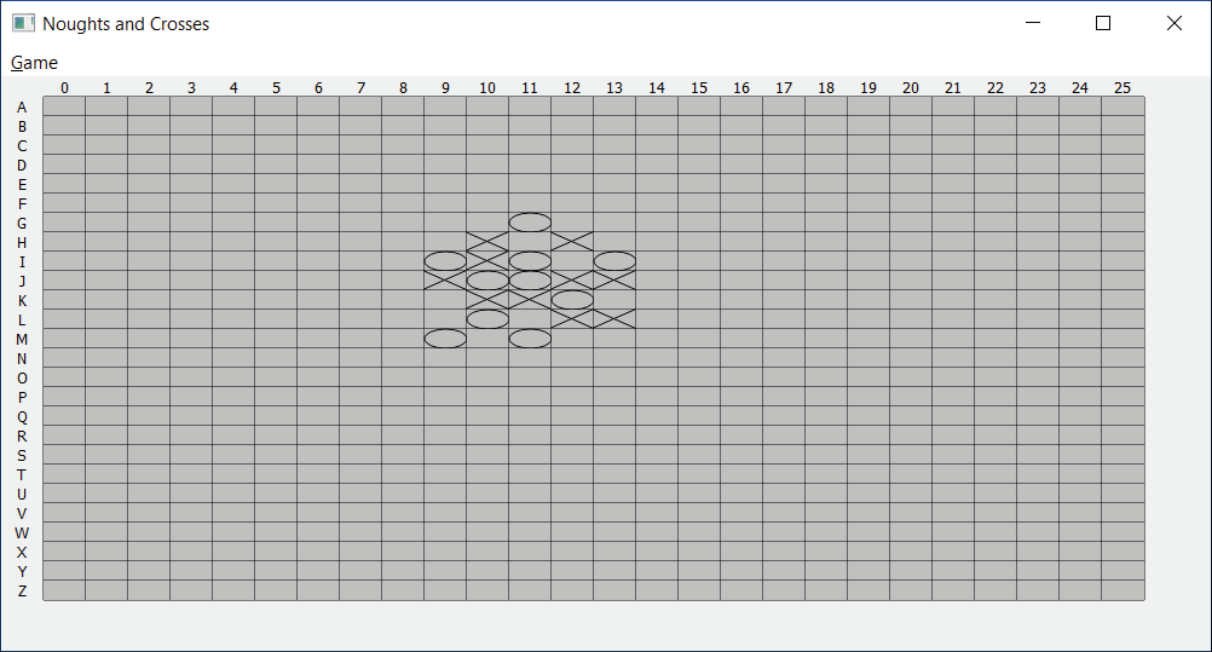
\includegraphics[width=0.9\textwidth]{images/p336_i03.png}\end{center}

\section{小结}

本章我们开发了奥赛罗棋和圈叉棋这两个游戏。我们初步接触了博弈论，并开发了一个游戏棋盘，玩家在其中轮流添加自己的棋子。在奥赛罗棋中，我们开发了为每一步统计待翻转棋子数量的方法；在圈叉棋中，我们开发了识别是否有玩家成功把五枚棋子排成一行的方法——如果有，我们就宣布该玩家为获胜者。

在第 8 章「计算机对弈」中，我们将开发这两个游戏的更高级版本，让计算机与人类对弈。
